\documentclass[a4paper,french,11pt]{article}

%%%% paquetages %%%%
\usepackage[french]{babel}  %d?finition de la langue
\usepackage[utf8]{inputenc} %d?finition de l'encodage
\usepackage{fullpage} %pour r?duire les marges
\usepackage{graphicx} %pour figures

%%%% param?tres de la commande \maketitle (titre) %%%%
\title{Titre du document}
\author{auteurs}
\date{date}

\begin{document}

\maketitle


\tableofcontents
\newpage

\section{Question 1}

Mon code C :

\begin{verbatim} %comme a la machine avec tous les blancs
//blabla
int main() {
for int i = j++;
  malloc;
  while;
  case
    break switch
\end{verbatim}

\section{Question 2}

\subsection{Formules}

Mes formules math?matiques $\int_{0}^{T}\cos(2\Pi nt)dt$.

Mes formules math?matiques centr?es :
$$g(t) = \frac{c}{2} + \sum_{n=1}^{+\infty}a_n \cos \left(\frac{2\Pi n}{T}t\right) + \sum_{n=1}^{+\infty}b_n \sin(2\Pi nft)$$

\subsection{Figures}

Mes figures, comme \ref{fig-toto} au format pdf

\begin{figure}[htbp] %here top bottom past page
\centering
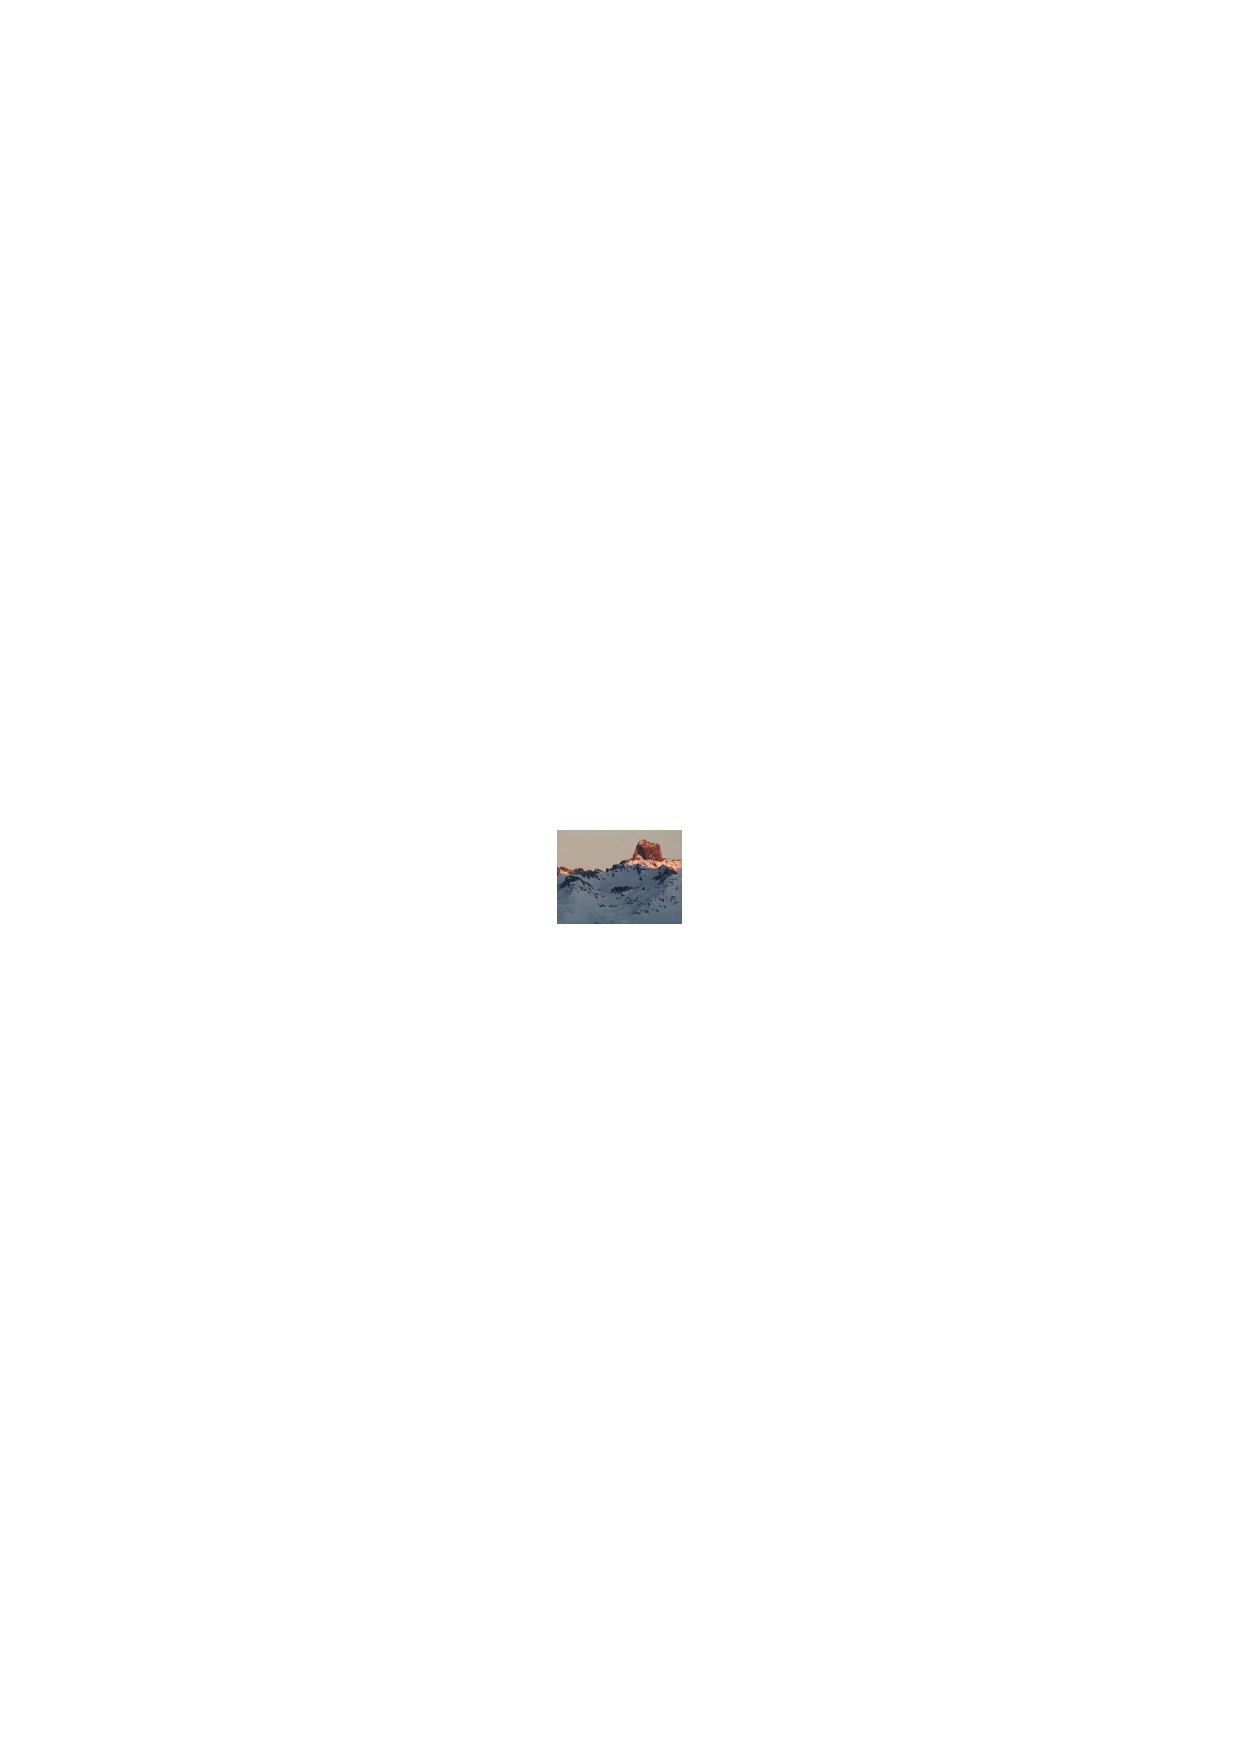
\includegraphics[width=0.3\linewidth]{./page1}
\caption{An example of figure. }
\label{fig-toto}
\end{figure}


\subsection{Tables}
\label{sec-tab}
Mes tableaux comme \ref{matable} dans la section \ref{sec-tab}:

\begin{table}[htp] %TODO d ?
\caption{Ma table}
\begin{center}
\begin{tabular}{|c|r|} %center right left ...
\hline 
Nom&Prenom\\ \hline \hline 
Toto & Bernard \\
Tutu & JB \\ \hline 

\end{tabular}
\end{center}
\label{matable}
\end{table}%

Je vous laisse d\'ecouvrir Bibtex et les citations. Attention ne jamais utiliser LaTeX comme Word : le compilateur doit faire la mise en page, pas vous ! Si vous faites la mise en page, {\bf LibreOffice} est {\it BEAUCOUP} plus performant.

\end{document}
